\usepackage[portuguese]{babel}
\usepackage{graphicx}

\begin{question}
 
O gráfico representa a temperatura de uma amostra de massa 115 gramas de determinado metal, inicialmente sólido, em função da quantidade de calor por ela absorvida. Determine o calor latente de fusão desse metal, em cal/g. \textit{Arredonde sua resposta para 1 casa decimal.}

\begin{figure}
  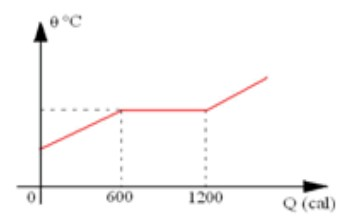
\includegraphics[height=10cm]{../../figuras/Q15CalL.jpg}
\end{figure}

\end{question}

\begin{solution}
  
  5.2 cal/g
  
\end{solution}

%% META-INFORMATION
%% \extype{num}
%% \exsolution{5.2}
%% \exname{Q15CalL}
%% \extol{0.1}
